\documentclass[11pt]{article}
\usepackage{graphicx}
\usepackage{multirow}
\usepackage{amsmath,amssymb,amsfonts}
\usepackage{amsthm}
\usepackage[title]{appendix}
\usepackage{xcolor}
\usepackage{textcomp}
\usepackage{booktabs}
\usepackage{listings}
\usepackage{url}
\usepackage[LGR,T1]{fontenc}
\usepackage[utf8]{inputenc}
\usepackage{alphabeta}
\usepackage[a4paper,margin=2.4cm]{geometry}
\usepackage{caption}
\usepackage{enumitem}
\usepackage[hidelinks]{hyperref}
\captionsetup{font=small,labelfont=bf}
\setlength{\parskip}{0.4em}
\setlength{\parindent}{0pt}
\newcommand{\euro}{\texteuro}
\definecolor{srcgray}{gray}{0.35}
\newcommand{\src}[1]{{\footnotesize\color{srcgray}[\textit{πηγή:} #1]}}

\title{\textbf{Δημόσια Ανώτατη Εκπαίδευση στην Ελλάδα, 2015--2025:\\
Ζήτηση, Κενές Θέσεις και Εισαγωγές σε Μη Εθνικά Πανεπιστήμια}\\[4pt]
\large Δομημένη Εμπειρική Έκθεση, «Πυξίδα Πανεπιστημίου»}
\author{Εικόνα Σύνοψης Δεδομένων: 21 Ιουλίου 2026}
\date{}

\begin{document}
\maketitle

\begin{abstract}
\noindent
Αυτή η έκθεση συνθέτει 10 χρόνια επίσημων δεδομένων εισαγωγών για τα ελληνικά
πανεπιστήμια (618 τμήματα, 10.290 εγγεγραμμένοι φοιτητές ανά τμήμα/έτος/πεδίο,
data.gov.gr, Υπουργείο Παιδείας) για να εξαγάγει τρία εμπειρικά αποτελέσματα και
ένα αρνητικό αποτέλεσμα. Πρώτον, οι κενές θέσεις καθορίζονται από τη ζήτηση και
όχι από το κόστος διαμονής (συντελεστής μερικής συσχέτισης $-0{,}35$ ελέγχοντας
για μεταβλητές αναφοράς, Πείραμα Φυσικού Περιεχομένου Κρήτης). Δεύτερον, τα μη
εθνικά διαπιστευμένα πανεπιστήμια (ΝΠΠΕ, ν.5094/2024) βρίσκονται σε περιοχές με
την υψηλότερη δημόσια ζήτηση και όχι σε περιοχές όπου υπάρχουν κενές θέσεις.
Τρίτον, η μείωση της περιφερειακής αξίας έχει σημαντικό οικονομικό αντίκτυπο
(περίπου 31,7 εκατομμύρια \euro\ ετησίως). Αρνητικό αποτέλεσμα: Ο περιφερειακός
πλούτος δεν προβλέπει κορεσμό ($r=0{,}13$, $p\approx0{,}40$). Κάθε αριθμός είναι
αναπαραγώγιμος τόσο σε σημεία που βασίζονται στο API όσο και σε τελικά σημεία, και
οποιαδήποτε ερμηνεία χαρακτηρίζεται σαφώς ως ερμηνεία και περιορίζεται από τα
δεδομένα.
\end{abstract}

\section{Βασικά δεδομένα και μεθοδολογικά σημεία}

\textbf{Βασικά δεδομένα.} Δημόσια δεδομένα data.gov.gr (Υπουργείο Παιδείας):
Κριτήρια εισαγωγής, ποσοστά αποδοχής/εισαγωγής, προτίμηση, στατιστικά στοιχεία
βαθμολογίας. Κανονικοποιημένο σε έναν μόνο πίνακα χρησιμοποιώντας σταθερούς
κωδικούς τμημάτων και έναν πίνακα μετασχηματισμού για μετονομασία/συγχώνευση
(Κύρια ασυνέχεια: Ενοποίηση ΤΕΙ 2018--2019).

\textbf{Διάστημα.} 2015--2019 και 2024--2025. Τα κενά στην περίοδο 2020--2023 δεν
υπάρχουν στα επίσημα δημόσια δεδομένα και επομένως εμφανίζονται ως κενά χωρίς
παρεμβολή.

\textbf{Κατηγορίες ανάλυσης.} Με βάση το ΓΕΛ90 (Γενική Σειρά Ημερησίων ΓΕΛ).
Πλαίσιο NUTS-3 της Eurostat (Τουρισμός, ΑΕΠ κατά κεφαλήν, πληθυσμός, δαπάνη ανά
φοιτητή). Εξαιρούνται οι στρατιωτικές/αστυνομικές ακαδημίες.

\begin{table}[h]\centering
\caption{Πηγές δεδομένων ανά μεταβλητή}
\small
\begin{tabular}{@{}lll@{}}
\toprule
Μεταβλητή & Πηγή & Έτος \\ \midrule
Σχολεία, Εγγεγραμμένοι φοιτητές, Κενές θέσεις & data.gov.gr (Υπ. Παιδείας) & 2015--2025 \\
Μέγιστη προτίμηση (Ζήτηση) & data.gov.gr Μηχανογραφημένο & 2024--2025 \\
ΑΕΠ κατά κεφαλήν, Πληθυσμός (NUTS-3) & Eurostat & 2021--2023 \\
Δαπάνες ανά μαθητή & Eurostat \texttt{educ\_uoe\_fini04} & 2012--2023 \\
Σχολικά δίδακτρα, προγράμματα ΝΠΠΕ & Έκθεση Έρευνας §4 & 2024 \\
\bottomrule
\end{tabular}
\end{table}

\section{Τα ποσοστά κενών θέσεων καθορίζονται από τη ζήτηση, όχι από τα προβλήματα στέγασης}

\begin{figure}[h]\centering
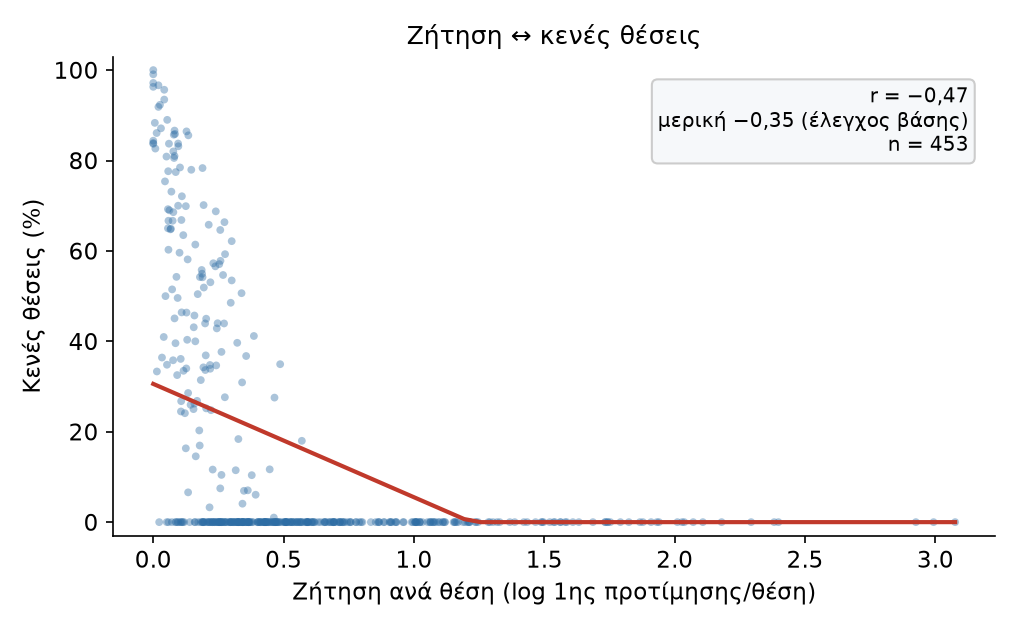
\includegraphics[width=0.72\linewidth]{fig_pyxida_demand.png}
\caption{Ζήτηση ανά χωρητικότητα (Μέγιστη προτίμηση/λογάριθμος χωρητικότητας)
έναντι κενών θέσεων, ΓΕΛ90 2025 ($n=453$). Αρνητική συσχέτιση $r=-0{,}47$· μερική
συσχέτιση που ελέγχει για τη μεταβλητή αναφοράς $-0{,}35$. \src{University Compass
Database, endpoint \texttt{/stats/demand}}}
\end{figure}

Η ζήτηση ανά θέση (η προτίμηση θέσης που καταχωρείται από τον υπολογιστή,
ανεξάρτητα από τους τελικούς αιτούντες) δείχνει αρνητική συσχέτιση ($r=-0{,}47$)
με τα ποσοστά κενών θέσεων. Δεδομένου ότι η ζήτηση συσχετίζεται επίσης με τη
μεταβλητή αναφοράς πριν από την ΕΒΕ ($r=0{,}60$), η υπολογισμένη μερική συσχέτιση
που ελέγχει για τη μεταβλητή αναφοράς είναι $-0{,}35$. Παρά τον παράγοντα
συγχύσεως της μεταβλητής αναφοράς, η ζήτηση δείχνει την ισχυρότερη συσχέτιση με τα
ποσοστά κενών θέσεων.

\textbf{Φυσικό πείραμα (Κρήτη).} Όταν τα ενοίκια στο νησί είναι σχεδόν σταθερά, τα
ποσοστά κενών θέσεων ποικίλλουν περίπου τρεις φορές (Χανιά περίπου 39\%, Ρέθυμνο
περίπου 28\%, Ηράκλειο περίπου 13\%). Εάν τα προβλήματα στέγασης ήταν η αιτία,
τέτοιες διακυμάνσεις δεν θα συνέβαιναν με το σταθερό κόστος στέγασης. Τα πραγματικά
δεδομένα ενοικίων (Numbeo/Spitogatos) επιβεβαίωσαν ότι τα ενοίκια δεν προβλέπουν
τα ποσοστά κενών θέσεων. \emph{(Στατιστικός τύπος: Αυτή είναι μόνο μια συσχέτιση·
η αιτιότητα δεν έχει αποδειχθεί.)}

\section{Πεδία εισαγωγής για μη εθνικά πανεπιστήμια}

\begin{figure}[h]\centering
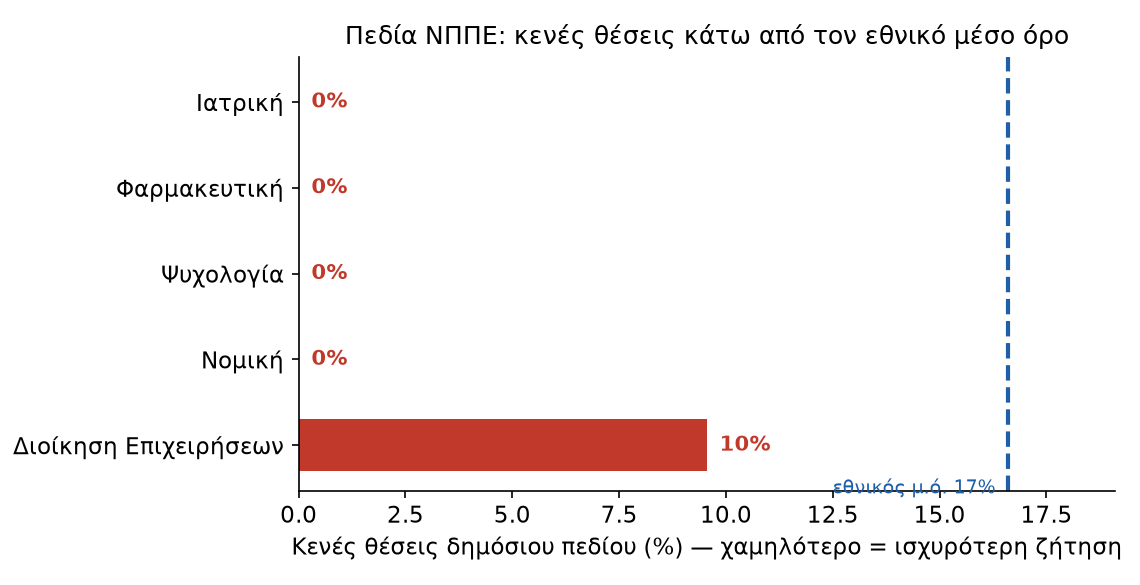
\includegraphics[width=0.78\linewidth]{fig_pyxida_intent.png}
\caption{Σύγκριση του μέσου ποσοστού κενών θέσεων στον δημόσιο τομέα για κάθε
πρόγραμμα ΝΠΠΕ με τον εθνικό μέσο όρο (17\%). Χαμηλότερη τιμή = ισχυρότερη δημόσια
ζήτηση. \src{University Compass Database, endpoint \texttt{/nppe/intent}}}
\end{figure}

Και τα πέντε προγράμματα που είναι πιστοποιημένα από το ΝΠΠΕ είναι του δημόσιου
τομέα, με ποσοστά κενών θέσεων κάτω από τον εθνικό μέσο όρο (17\%). Η Ιατρική, η
Φαρμακευτική, η Ψυχολογία και η Νομική έχουν ποσοστά κενών θέσεων 0\%, ενώ η
Διοίκηση Επιχειρήσεων έχει ποσοστό 10\%. Με άλλα λόγια, η ιδιωτική προσφορά
συγκεντρώνεται σε περιοχές με την ισχυρότερη δημόσια ζήτηση (δηλαδή, σε
μητροπολιτικές περιοχές υψηλού κύρους) και δεν συγκεντρώνεται σε περιοχές με
κενές θέσεις.

\textbf{Κόστος για τους αιτούντες.} Ένας φοιτητής με 17.500 μόρια απορρίπτεται και
από τις επτά δημόσιες ιατρικές σχολές (η πλησιέστερη Ιατρική Σχολή στην
Αλεξανδρούπολη έχει $-475$ μόρια). Η μόνη εναπομένουσα οδός είναι ένα ιδιωτικό
πανεπιστήμιο, το οποίο κοστίζει 162.000\,\euro\ (27.000\,\euro\ ετησίως) για την
απόκτηση εξαετούς πτυχίου. \emph{Ερμηνεία εντός των ορίων των δεδομένων:} Αυτό το
μοτίβο είναι συνεπές με τη στρατηγική εμπορική είσοδο σε μια ισχυρή δημόσια αγορά.
Αυτό δεν καταδεικνύει νομοθετική πρόθεση. Αυτό είναι πέρα από το πεδίο εφαρμογής
των στατιστικών και δεν υποστηρίζεται.

\textbf{Το κόστος για τον υποψήφιο.} Ένας μαθητής με 17.500 μόρια αστοχεί και τις
επτά δημόσιες σχολές Ιατρικής (εγγύτερη $-475$ μόρια, Αλεξανδρούπολη). Η μόνη
εναπομείνασα διαδρομή είναι η ιδιωτική, με \textbf{162.000\,\euro} για το εξαετές
πτυχίο (27.000\,\euro/έτος). \emph{Ερμηνεία εντός των ορίων των δεδομένων:} το
μοτίβο είναι \emph{συμβατό με} στοχευμένη εμπορική είσοδο σε ισχυρές δημόσιες
αγορές. Δεν αποδεικνύει νομοθετική πρόθεση, αυτό μένει εκτός στατιστικής
εμβέλειας και δεν διεκδικείται.

\section{Το δημοσιονομικό αποτύπωμα της περιφερειακής απαξίωσης}

\[
\underbrace{10{.}628}_{\text{κενές θέσεις ΓΕΛ90 2025}}\ \times\
\underbrace{2{.}984\,\euro}_{\substack{\text{δημόσια δαπάνη/φοιτητή}\\ \text{Eurostat 2023}}}\ =\
\boxed{\ \sim 31{,}7\ \text{εκ.}\,\euro/\text{έτος}\ }\ \approx 127\ \text{εκ.}\,\euro\ \text{ανά τετραετία}
\]

\emph{Επιφύλαξη (ρητή).} Το μέγεθος εκτιμά τη δημόσια χρηματοδότηση που
\emph{αντιστοιχεί} κατ' αναλογία εγγραφών στις κενές θέσεις, όχι το οριακό
κόστος ή την πραγματική εξοικονόμηση. Η δαπάνη ανά φοιτητή είναι πραγματικό
στοιχείο Eurostat (\texttt{educ\_uoe\_fini04}), όχι εκτίμηση. Οι κενές θέσεις
συγκεντρώνονται στη μη μητροπολιτική περιφέρεια (Ευρυτανία $\sim$96\%, Δράμα
$\sim$93\%, απομακρυσμένα νησιά $>$40\%), ενώ τα μητροπολιτικά κέντρα γεμίζουν.

\section{Αρνητικό αποτέλεσμα: ο πλούτος δεν εξηγεί την πληρότητα}

Ελέγξαμε την κοινή αφήγηση «οι πλούσιες περιοχές γεμίζουν τις σχολές τους». Η
συσχέτιση ΑΕΠ/κατοίκου--πληρότητας σε επίπεδο περιφέρειας είναι $r=0{,}13$,
$p\approx0{,}40$ ($n=42$), \textbf{μη στατιστικά σημαντική}. Ο περιφερειακός
πλούτος δεν προβλέπει την πληρότητα.

\emph{Οικολογικό σφάλμα (ρητή προειδοποίηση):} πρόκειται για περιφερειακό μέτρο·
δεν μετρά ατομικό οικογενειακό εισόδημα και δεν τεκμηριώνει αποκλεισμό φτωχών
φοιτητών. Το αναφέρουμε ως αρνητικό αποτέλεσμα ακριβώς επειδή τα δεδομένα δεν το
επιβεβαίωσαν, η δημοσίευση αρνητικών αποτελεσμάτων είναι μέρος της
μεθοδολογικής εντιμότητας.

\section{Πρόβλεψη βάσεων: το μηχανιστικό μοντέλο ΕΒΕ κερδίζει το benchmark}

Αρχικά, σε backtesting με το κενό 2020--2023 παρόν, κανένα χρονοσειριακό μοντέλο
δεν ξεπερνούσε τη μεταφορά της περυσινής τιμής (carry-forward). Αφού
συμπληρώθηκε το κενό (δεδομένα aeitei.gr) και μοντελοποιήθηκε ρητά ο μηχανισμός
ΕΒΕ, η εικόνα άλλαξε. Το κλειδί που επαληθεύσαμε στα δεδομένα είναι ότι το
κατώφλι ΕΒΕ κάθε τμήματος ισούται με $\text{τιμή αναφοράς πεδίου} \times
\text{συντελεστή τμήματος}$: εντός κάθε πεδίου-έτους ο λόγος
$\text{κατώφλι}/\text{συντελεστή}$ είναι σχεδόν σταθερός (απόκλιση 0,04--3,2\%).

Σε backtest 2024$\to$2025 (446 τμήματα), το \textbf{μηχανιστικό μοντέλο ΕΒΕ}
είναι το μόνο που νικά το carry-forward benchmark και στους δύο στόχους: ΜΑΕ
βάσης 375 έναντι 400 μόρια, ΜΑΕ εισακτέων 10{,}4 έναντι 11{,}7. Το gradient
boosting κερδίζει οριακά μόνο στη βάση (397) και χάνει στους εισακτέους (14{,}7)·
δεν αποστέλλεται. Τα δεδομένα είναι πολύ μικρού $N$ και πολύ μηχανιστικά για να
ανταμείψουν τα εύκαμπτα μοντέλα μηχανικής μάθησης.

\begin{figure}[h]\centering
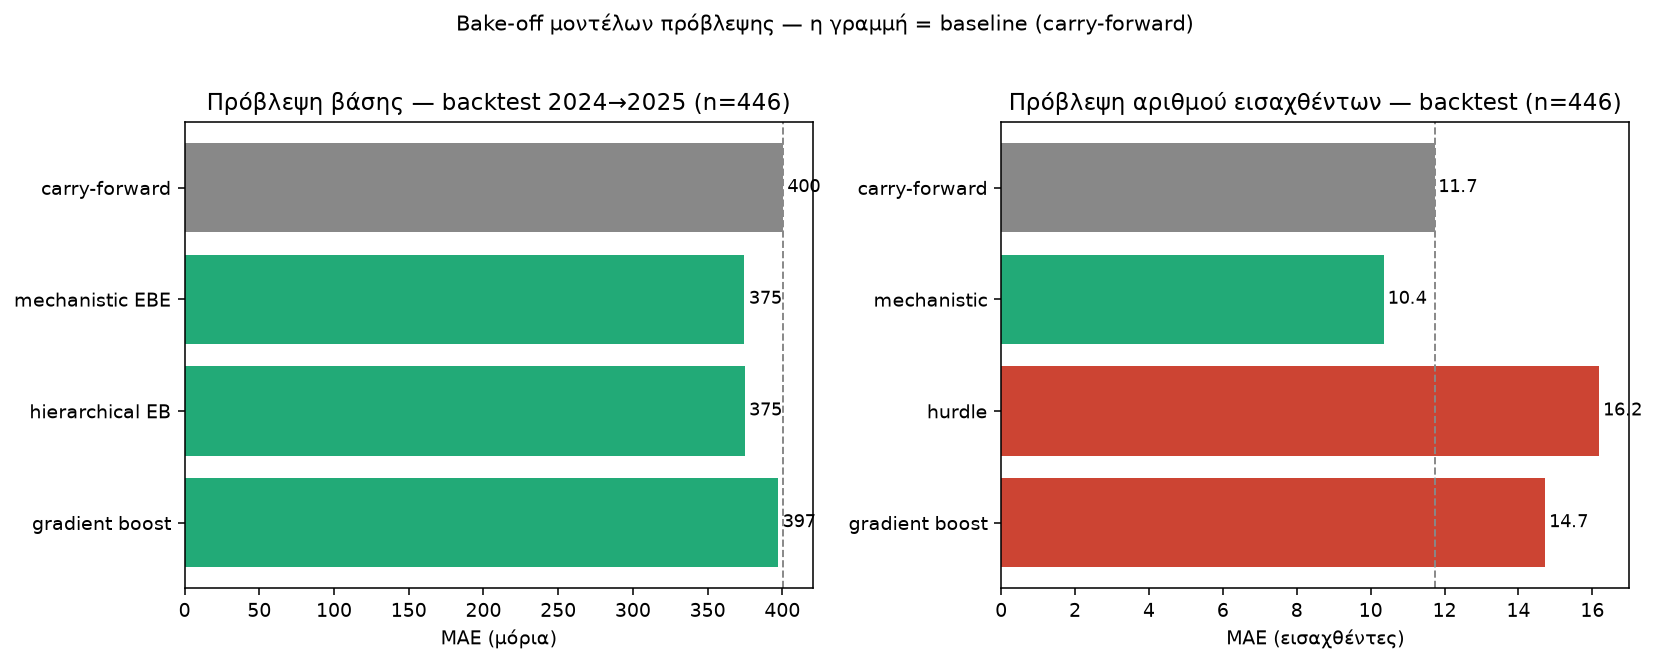
\includegraphics[width=\textwidth]{model_bakeoff.png}
\caption{Σύγκριση σφάλματος (ΜΑΕ) πέντε μοντέλων, backtest 2024$\to$2025. Η
διακεκομμένη γραμμή είναι το carry-forward benchmark. Μόνο το μηχανιστικό μοντέλο
ΕΒΕ νικά και στους δύο στόχους.}
\end{figure}

Το μοντέλο βλέπει ρητά δύο θεσμικούς μοχλούς --- την τιμή αναφοράς πεδίου
(επίδοση εξετάσεων· 2026: 1ο $-0{,}8\%$, 2ο $+6{,}6\%$, 3ο $+2{,}8\%$, 4ο
$-1{,}6\%$) και τον συντελεστή τμήματος (ΦΕΚ). Είναι όμως τυφλό σε δύο φαινόμενα
ζήτησης, τα οποία προσθέσαμε ως χωριστά στρώματα:

\begin{itemize}[leftmargin=1.4em,itemsep=1pt]
\item \textbf{Υποκατάσταση εντός Φιλοσοφικής Σχολής.} Η κοινή δεξαμενή υποψηφίων
Φιλολογίας--Ιστορίας--Φιλοσοφίας σημαίνει ότι ένα νέο ελκυστικό πρόγραμμα τραβάει
ζήτηση από τα αδέλφια τμήματα. Το \emph{μοντέλο συστάδας} (πρόβλεψη του συνόλου
της σχολής, κατανομή μεριδίων κατά ελκυστικότητα) νικά το benchmark κατά 27\%
(ΜΑΕ 18{,}1 έναντι 24{,}9) στα 15 τμήματα των πέντε Φιλοσοφικών Σχολών.
\item \textbf{Γεωγραφική υποκατάσταση.} Οι υποψήφιοι που χάνουν επιλεξιμότητα σε
ένα τμήμα κατευθύνονται στα κοντινότερα ηπειρωτικά τμήματα (μοντέλο βαρύτητας με
απόσβεση απόστασης και ποινή θαλάσσιου περάσματος), όχι σε νησιωτικά ή μακρινά.
\end{itemize}

\begin{figure}[h]\centering
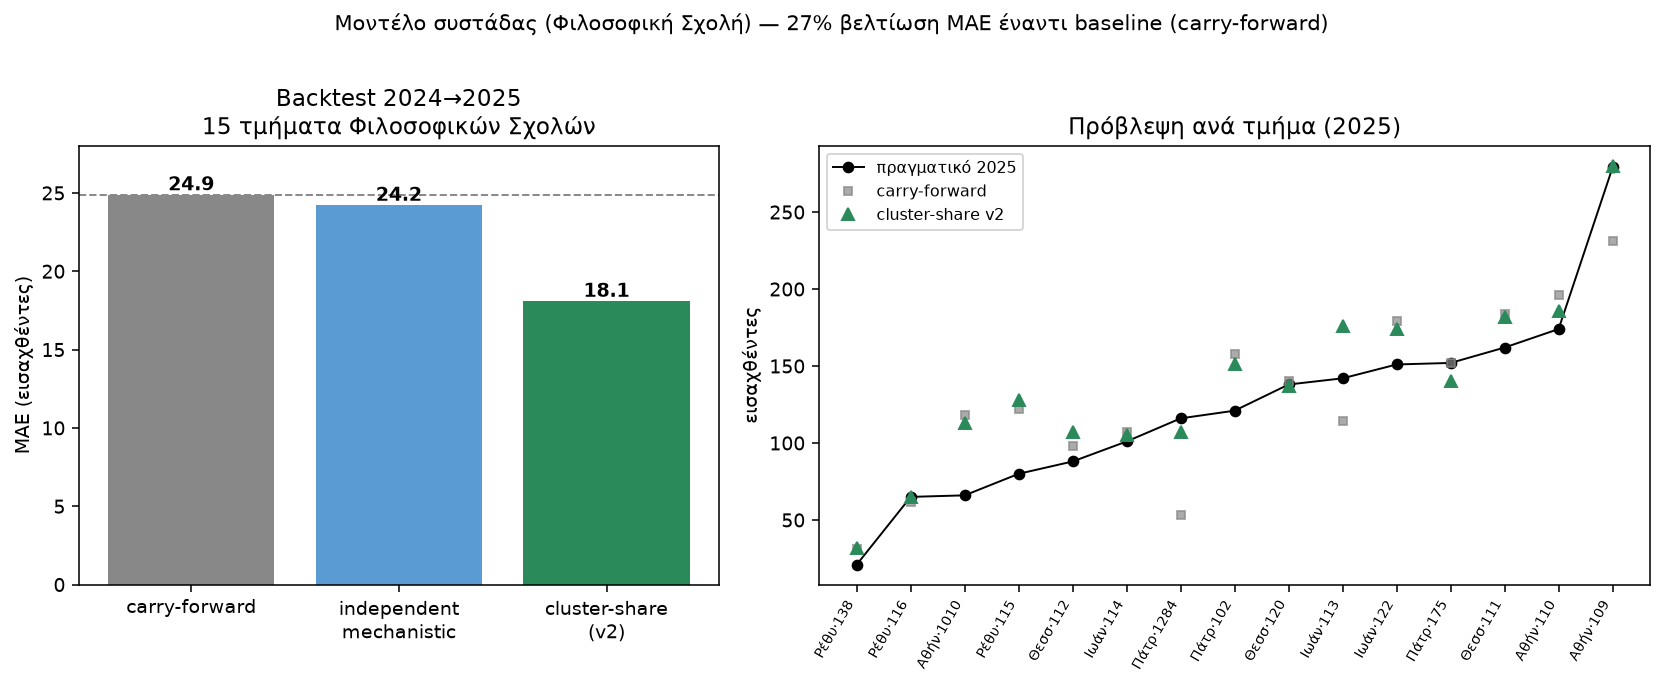
\includegraphics[width=0.92\textwidth]{cluster_model.png}
\caption{Μοντέλο συστάδας για τις Φιλοσοφικές Σχολές: 27\% βελτίωση ΜΑΕ έναντι
carry-forward, με περιορισμό των υπερβολών του ανεξάρτητου μοντέλου.}
\end{figure}

\begin{figure}[h]\centering
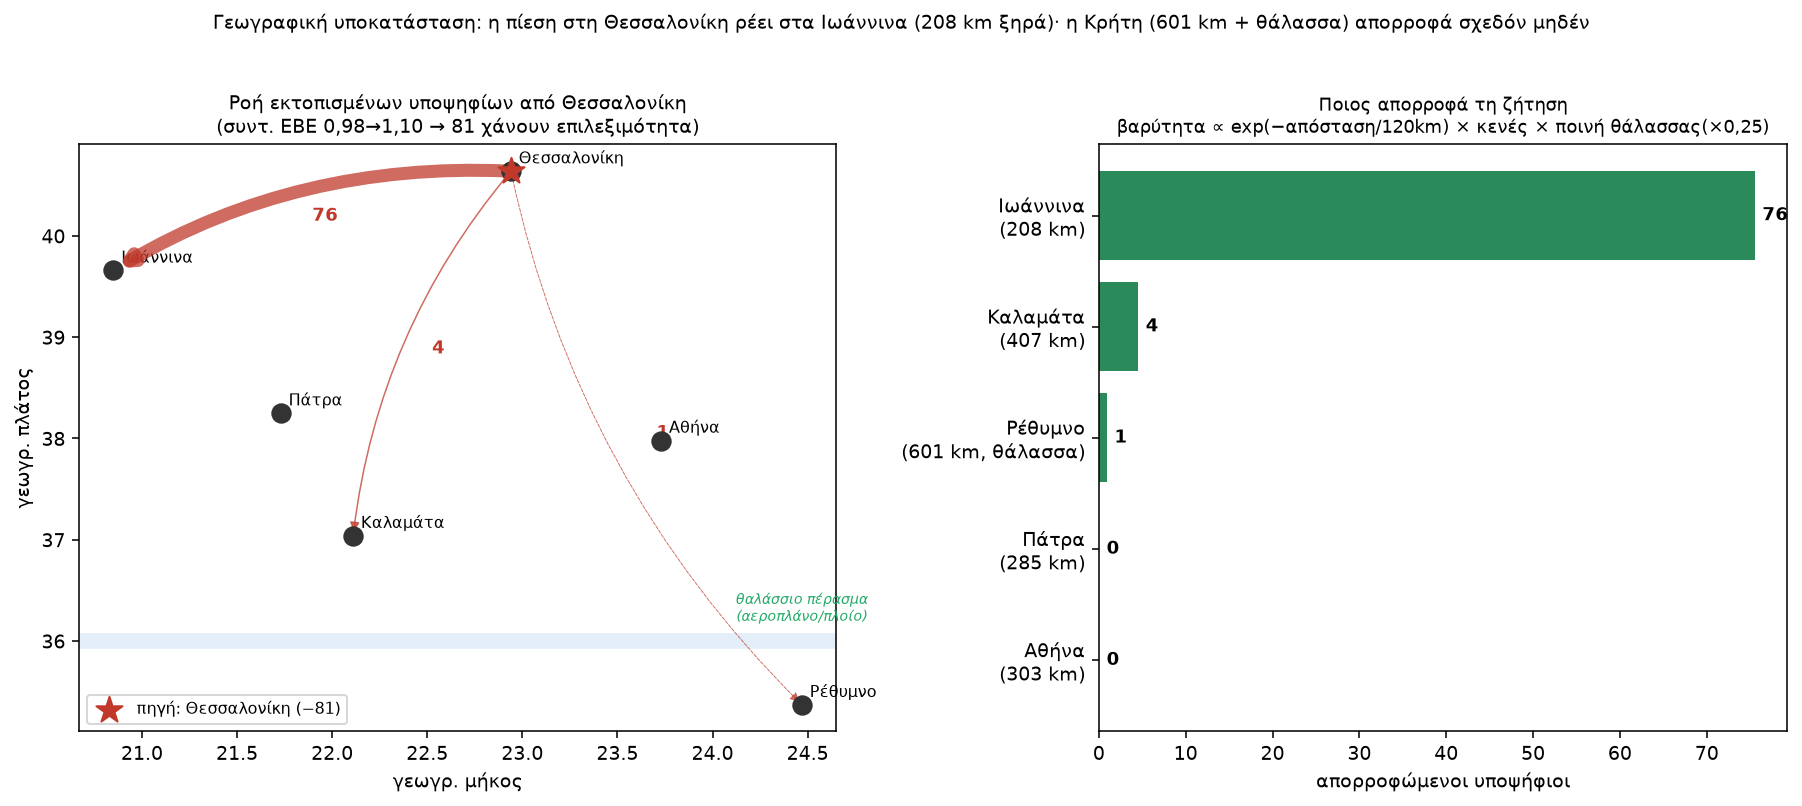
\includegraphics[width=\textwidth]{gravity_substitution.png}
\caption{Γεωγραφική υποκατάσταση: η πίεση σε ένα τμήμα ρέει στα κοντινά ηπειρωτικά
τμήματα (π.χ. Θεσσαλονίκη$\to$Ιωάννινα, 208 km ξηρά), όχι στην Κρήτη (601 km +
θάλασσα + ακριβότερο ενοίκιο).}
\end{figure}

Η προβλεπόμενη βάση ορίζεται ως $\max(\text{εκτίμηση ΕΒΕ},\ \text{demand model})$
και συνοδεύεται πάντα από διάστημα εμπιστοσύνης· ουδέποτε παρουσιάζεται σημειακή
πρόβλεψη «η βάση θα είναι X». Οι δύο μοχλοί ζήτησης (ένταση νέου προγράμματος,
ένταση γεωγραφικής μεταφοράς) δικαιολογούνται δομικά αλλά \emph{δεν} είναι
στατιστικά βαθμονομημένοι --- δεν υπήρξε αντίστοιχο γεγονός στο ιστορικό. Τα
πραγματικά στοιχεία 2026 αποτελούν τον τελικό κριτή.

\section{Περιορισμοί}
\begin{itemize}[leftmargin=1.4em,itemsep=1pt]
\item Κενό 2020--2023 απόν από τα επίσημα ανοικτά δεδομένα· συμπληρώθηκε από
δευτερογενή πηγή (aeitei.gr, βάσεις + ΕΒΕ, χωρίς θέσεις/εισαχθέντες), με ρητή
σήμανση προέλευσης.
\item Μικρό $N$ ανά σειρά τμήματος $\Rightarrow$ προτίμηση σε pooling/μηχανισμό
έναντι ευέλικτων μοντέλων· ένα καθαρό πρόσφατο βήμα (2024$\to$25) περιορίζει την
ισχύ του backtest.
\item ΑΕΠ/κάτοικο ως proxy κόστους· πραγματικά ενοίκια επιβεβαίωσαν το εύρημα.
\item «Πρόθεση» ΝΠΠΕ: ερμηνεία συμβατή με τα δεδομένα, όχι αιτιακή ταυτοποίηση.
\item Προβολή 2030: σενάριο υπό όρους, όχι πρόβλεψη· διαστήματα φραγμένα στο $[0,1]$.
\end{itemize}

\section{Αναπαραγωγιμότητα και παραπομπή}

Κάθε σχήμα αντιστοιχεί σε endpoint (\texttt{/stats/demand}, \texttt{/nppe/intent},
\texttt{/stats/abandonment-cost}, \texttt{/stats/wealth-fill},
\texttt{/stats/projection}). Η βάση ξαναχτίζεται με μία εντολή από τα raw
δεδομένα. Προτεινόμενη παραπομπή: \emph{Πυξίδα ΑΕΙ, στιγμιότυπο 2026-07-21· πηγές:
data.gov.gr (Υπ. Παιδείας), Eurostat.}

\begin{thebibliography}{9}
\bibitem{minedu} Υπουργείο Παιδείας, Θρησκευμάτων \& Αθλητισμού, Ανοικτά
δεδομένα βάσεων και μηχανογραφικών, \url{https://data.gov.gr}.
\bibitem{eurostat} Eurostat, \emph{Education finance statistics}
(\texttt{educ\_uoe\_fini04}) και περιφερειακοί λογαριασμοί NUTS-3.
\bibitem{nppe} Ν.5094/2024, Ίδρυση και λειτουργία μη κρατικών, μη κερδοσκοπικών
Ανώτατων Εκπαιδευτικών Ιδρυμάτων (ΝΠΠΕ).
\bibitem{ebe} Ν.4777/2021, Ελάχιστη Βάση Εισαγωγής (ΕΒΕ).
\bibitem{fek2026} ΥΑ Φ.253/160742/Α5/10-12-2025, ΦΕΚ Β' 6782/16-12-2025
(συντελεστές ΕΒΕ ανά τμήμα, έτος 2026).
\bibitem{aeitei} aeitei.gr, ιστορικό βάσεων και ΕΒΕ 2015--2026 (δευτερογενής
πηγή για το κενό 2020--2023).
\end{thebibliography}

\end{document}
